\documentclass{article}

\usepackage{times}
\usepackage{graphicx} % more modern
\usepackage{subfigure} 
\usepackage{natbib}
\usepackage{algorithm}
\usepackage{algorithmic}
\usepackage{hyperref}
\newcommand{\theHalgorithm}{\arabic{algorithm}}
\usepackage[accepted]{icml2016}


\usepackage{comment}

\icmltitlerunning{LSTM for Text Generation and Classification}
%\yrcite{} if named otherwise \cite
\begin{document} 

\twocolumn[
\icmltitle{LSTM for Text Generation and Classsification}
\icmlauthor{Your Name}{email@yourdomain.edu}
\icmlauthor{Your CoAuthor's Name}{email@coauthordomain.edu}

\vskip 0.3in
]

\begin{abstract} 
bla
\end{abstract} 
\medskip
\section{Introduction}
\clearpage
\section{Citations and References} 

\bibliography{example_paper}
\bibliographystyle{icml2016}

\end{document} 


%examples
\begin{figure}[ht]
\vskip 0.2in
\begin{center}
\centerline{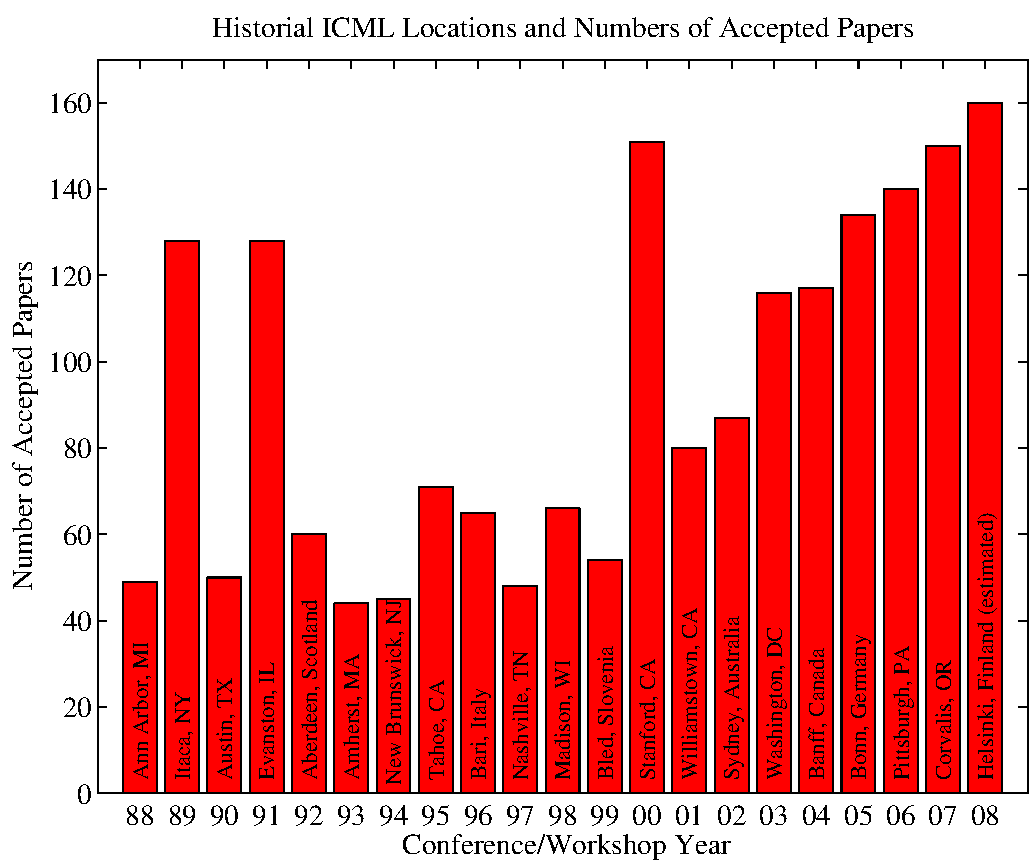
\includegraphics[width=\columnwidth]{icml_numpapers}}
\caption{}
\label{icml-historical}
\end{center}
\vskip -0.2in
\end{figure} 

\begin{algorithm}[tb]
   \caption{Bubble Sort}
   \label{alg:example}
\begin{algorithmic}
   \STATE {\bfseries Input:} data $x_i$, size $m$
   \REPEAT
   \STATE Initialize $noChange = true$.
   \FOR{$i=1$ {\bfseries to} $m-1$}
   \IF{$x_i > x_{i+1}$} 
   \STATE Swap $x_i$ and $x_{i+1}$
   \STATE $noChange = false$
   \ENDIF
   \ENDFOR
   \UNTIL{$noChange$ is $true$}
\end{algorithmic}
\end{algorithm}
 
\begin{table}[t]
\caption{Classification accuracies for naive Bayes and flexible 
Bayes on various data sets.}
\label{sample-table}
\vskip 0.15in
\begin{center}
\begin{small}
\begin{sc}
\begin{tabular}{lcccr}
\hline
\abovespace\belowspace
Data set & Naive & Flexible & Better? \\
\hline
\abovespace
Breast    & 95.9$\pm$ 0.2& 96.7$\pm$ 0.2& $\surd$ \\
Cleveland & 83.3$\pm$ 0.6& 80.0$\pm$ 0.6& $\times$\\
Glass2    & 61.9$\pm$ 1.4& 83.8$\pm$ 0.7& $\surd$ \\
Credit    & 74.8$\pm$ 0.5& 78.3$\pm$ 0.6&         \\
Horse     & 73.3$\pm$ 0.9& 69.7$\pm$ 1.0& $\times$\\
Meta      & 67.1$\pm$ 0.6& 76.5$\pm$ 0.5& $\surd$ \\
Pima      & 75.1$\pm$ 0.6& 73.9$\pm$ 0.5&         \\
\belowspace
Vehicle   & 44.9$\pm$ 0.6& 61.5$\pm$ 0.4& $\surd$ \\
\hline
\end{tabular}
\end{sc}
\end{small}
\end{center}
\vskip -0.1in
\end{table}
